\documentclass[12pt,letterpaper]{article}

\usepackage[utf8]{inputenc}
\usepackage[spanish,es-nodecimaldot]{babel}
\usepackage{helvet}
\renewcommand{\familydefault}{\sfdefault}
\usepackage{setspace}
\setstretch{1.12}
\usepackage[margin=2cm]{geometry}
\usepackage{graphicx}
\graphicspath{{./images/}}
\usepackage{booktabs}
\usepackage{tabularx}
\usepackage{amssymb}
\usepackage{enumitem}
\usepackage{fancyhdr}
\usepackage{titlesec}
\usepackage{xcolor}
\usepackage{xurl}
\usepackage{hyperref}

\hypersetup{
    colorlinks=true,
    linkcolor=black,
    citecolor=blue!70!black,
    urlcolor=cyan!70!black,
    pdftitle={Tarea 1: Definición y Validación del Problema - CD1201},
    pdfauthor={Equipo 13 (Walli-s): Felipe Colli, Agustín Concha, Benjamín Bascuñán, Diego Alvarado, Joaquín Pérez},
    pdfsubject={Información recopilada con asistencia de Google Antigravity}
}

% Formato de títulos compacto
\titleformat{\section}{\large\bfseries}{\thesection.}{0.4em}{}
\titleformat{\subsection}{\normalsize\bfseries}{\thesubsection.}{0.4em}{}
\titleformat{\subsubsection}{\small\bfseries}{\thesubsubsection.}{0.4em}{}
\titlespacing*{\section}{0pt}{0.8ex plus .1ex minus .1ex}{0.3ex}
\titlespacing*{\subsection}{0pt}{0.6ex plus .1ex minus .1ex}{0.2ex}
\titlespacing*{\subsubsection}{0pt}{0.5ex plus .1ex minus .1ex}{0.2ex}

% Encabezados y pies de página
\pagestyle{fancy}
\fancyhf{}
\fancyhead[L]{\footnotesize\textsf{CD1201 -- Proyecto de Innovación en Ingeniería y Ciencias}}
\fancyhead[R]{\footnotesize\textsf{Tarea 1 -- Equipo 13: Walli-s}}
\fancyfoot[L]{\footnotesize\textsf{FCFM -- Universidad de Chile}}
\fancyfoot[R]{\thepage}
\renewcommand{\headrulewidth}{0.4pt}
\renewcommand{\footrulewidth}{0.4pt}

% Sangría francesa para APA
\newcommand{\hangapa}{\par\noindent\hangindent=2em\hangafter=1}

\begin{document}

% =========================================================================
% PORTADA (1 PLANA ESTRICTA)
% =========================================================================
\begin{titlepage}
\thispagestyle{empty}
\begin{center}
    
\includegraphics[width=0.42\textwidth]{logo_fcfm.png}\\[0.6cm]
    
    {\Large\textbf{UNIVERSIDAD DE CHILE}}\\[0.15cm]
    {\large\textbf{FACULTAD DE CIENCIAS FÍSICAS Y MATEMÁTICAS}}\\[0.15cm]
    {\normalsize\textbf{ÁREA INGENIERÍA E INNOVACIÓN -- HÉLICE}}\\[0.15cm]
    {\small\textbf{CD1201 PROYECTO DE INNOVACIÓN EN INGENIERÍA Y CIENCIAS -- SECCIÓN 01}}\\[0.1cm]
    {\small\textbf{MÓDULO: ECOMAKER (ELECTRÓNICA Y MONITOREO AMBIENTAL)}}\\[1.2cm]

    \rule{\linewidth}{0.8mm}\\[0.3cm]
    {\LARGE\textbf{TAREA 1: DEFINICIÓN Y VALIDACIÓN DEL PROBLEMA}}\\[0.25cm]
    {\large\textbf{Proyecto: Wall-I's -- Sistema Robótico Autónomo de Limpieza y Tamizado Subsuperficial de Borde Costero}}\\[0.3cm]
    \rule{\linewidth}{0.8mm}\\[1.2cm]

    \begin{minipage}[t]{0.52\textwidth}
        \textbf{Equipo 13 (Walli-s):}\\[0.25cm]
        Felipe Colli Olea\\[0.15cm]
        Agustín Concha\\[0.15cm]
        Benjamín Bascuñán\\[0.15cm]
        Diego Alvarado\\[0.15cm]
        Joaquín Pérez
    \end{minipage}
    \hfill
    \begin{minipage}[t]{0.42\textwidth}
        \textbf{Equipo Docente:}\\[0.2cm]
        \textbf{Profesora:}\\ María Carolina Pino Ahumada\\[0.15cm]
        \textbf{Auxiliares:}\\ Vicente González\\ Millaray González\\[0.15cm]
        \textbf{Ayudante:}\\ Renato Planas
    \end{minipage}

    \vfill
    {\footnotesize\textit{*Nota: La información y antecedentes de este informe fueron recopilados con asistencia de Google Antigravity.}}\\[0.4cm]
    {\normalsize\textbf{Santiago de Chile, Septiembre de 2026}}
\end{center}
\end{titlepage}

\clearpage
\pagenumbering{arabic}
\setcounter{page}{2}

% =========================================================================
% SECCIÓN 1: CONTEXTUALIZACIÓN Y ORGANIZACIÓN DEL EQUIPO
% =========================================================================
\section{Contextualización de la Unidad 1 y Organización del Equipo}

\subsection{Contexto de la Unidad 1 y Enfoque del Desafío}
Chile cuenta con más de 6.500 kilómetros de línea de costa y cerca de 900 playas con alto valor ecológico y recreativo. No obstante, las playas de la zona central sufren una severa degradación ambiental debido a la acumulación de residuos antropogénicos concentrados en la temporada estival (Oceana Chile \& Científicos de la Basura, 2026). La Unidad 1 del curso CD1201 tiene como propósito central la definición y validación empírica en terreno de una problemática de ingeniería, conectando hallazgos empáticos, revisión bibliográfica y datos directos de usuarios y clientes para sustentar el desarrollo de soluciones en el módulo EcoMaker.

El proyecto \textbf{Walli-s} surge como la continuidad de nuestro equipo desde CD1100, abordando un vacío crítico no resuelto por las tecnologías actuales: la \textit{contaminación subsuperficial}. Mientras la limpieza municipal y los voluntariados retiran macrodesechos visibles en superficie, una vasta fracción de residuos pequeños (colillas de cigarro, tapas plásticas, envoltorios y vidrios rotos) se entierra bajo los primeros 5 a 10 cm de arena debido al viento, el tránsito peatonal y las mareas, originando riesgos permanentes de cortes, infecciones y daño ecológico.

\subsection{Conformación del Equipo, Afinidades y Roles}
El equipo de trabajo acordó unánimemente continuar de manera integrada con los cinco miembros originales, consolidando una dinámica caracterizada por la confianza y la complementariedad técnica:
\begin{itemize}[leftmargin=*, noitemsep, topsep=0pt]
    \item \textbf{Felipe Colli Olea (Líder Técnico, Hardware y Firmware):} Coordinación técnica, diseño electrónico en microcontroladores (ESP32), buses I2C/SPI, control de potencia y gestión de repositorios Git.
    \item \textbf{Agustín Concha (Coordinador de Terreno y Logística):} Planificación de salidas a terreno, coordinación con actores locales del balneario de El Tabo, levantamiento de observaciones y entrevistas.
    \item \textbf{Benjamín Bascuñán (Investigación y Estado del Arte):} Búsqueda de literatura científica, benchmarking de maquinaria existente (tractores BeachTech y robots) y análisis normativo (Leyes 21.100 y 21.368).
    \item \textbf{Diego Alvarado (Diseño Mecánico y Estructura):} Modelado 3D de chasis modular, cálculos de tracción en arena, diseño de compartimentos estancos y del mecanismo de cribado mecánico.
    \item \textbf{Joaquín Pérez (Visión Computacional e Inteligencia Artificial):} Implementación de modelos de detección visual de personas y obstáculos (YOLOv8), clasificación de residuos y análisis estadístico.
\end{itemize}

\subsection{Contrato de Equipo y Acuerdos de Funcionamiento}
Para asegurar una colaboración armónica, se formalizó el \textbf{Contrato de Equipo} (adjunto en el \textbf{Anexo A}). Este instrumento define valores rectores (responsabilidad compartida, comunicación proactiva y rigor técnico), canales oficiales (grupo de WhatsApp para coordinación cotidiana, Google Drive para documentos de trabajo y GitHub para código y bitácora) y acuerdos ``no negociables'' (revisión paritaria obligatoria de todo entregable y aviso con al menos 24 horas de antelación ante cualquier eventualidad personal).

% =========================================================================
% SECCIÓN 2: RESULTADOS DE ACTIVIDADES OBLIGATORIAS DE LA UNIDAD 1
% =========================================================================
\section{Resultados de Actividades Obligatorias de la Unidad 1}

\subsection{Observación de Campo y Registro en Terreno}
Se implementó un protocolo de observación estructurado en el borde costero de la comuna de El Tabo mediante transectos sistemáticos en tramos de 200 a 300 metros durante fines de semana, aplicando la metodología \textbf{AEIOU} (Actividades, Entornos, Interacciones, Objetos y Usuarios; detallada en el \textbf{Anexo D}). Los hallazgos revelaron tres fenómenos determinantes:
\begin{enumerate}[leftmargin=*, noitemsep, topsep=0pt]
    \item \textbf{Ceguera superficial:} Playas aparentemente limpias esconden gran cantidad de residuos al excavar entre 3 y 5 cm, con predominio de colillas (18\,\%), plásticos degradados (61\,\%) y vidrios (7\,\%).
    \item \textbf{Dinámica de mareas y reposición diurna:} El mar y el viento entierran rápidamente los desechos finos. Asimismo, los esfuerzos matutinos de limpieza se ven neutralizados hacia el mediodía por la afluencia de público y la escasez de contenedores cercanos.
    \item \textbf{Microbasurales perimetrales:} El viento arrastra residuos livianos hacia dunas y roqueríos, zonas donde la maquinaria pesada no tiene acceso físico.
\end{enumerate}

\subsection{Entrevista de Diagnóstico Inicial}
Como diagnóstico preliminar, se entrevistó a \textbf{Ana Jer} (56 años, residente de El Tabo desde 2018). Ana relató que el municipio realiza labores de aseo temprano en la mañana, pero resultan insuficientes: las cuadrillas manuales recogen únicamente residuos voluminosos (botellas y bolsas plásticas) usando palas de gran apertura, dejando intactas las colillas y astillas de vidrio. Señaló además que caminar descalzo genera una constante sensación de inseguridad para su familia, motivándola a recoger basura por cuenta propia.

\subsection{Matriz Aplicada del Problema (MAP)}
A partir de las observaciones de campo y revisión de fuentes secundarias, se formuló la \textbf{Matriz Aplicada del Problema (MAP)}, diferenciando entre \textbf{Usuarios} (quienes sufren el problema en su uso cotidiano) y \textbf{Clientes} (entidades con mandato legal y presupuesto de compra y mantenimiento).

\begin{table}[h!]
\centering
\footnotesize
\setstretch{1.02}
\begin{tabularx}{\textwidth}{p{3.2cm}X p{5.5cm}}
\toprule
\textbf{Segmento} & \textbf{Problema / Necesidad Crítica} & \textbf{Alternativas Actuales y Brecha} \\
\midrule
\textbf{Usuario:} Turistas, familias, niños y residentes del borde costero. & 
Necesitan recrearse y transitar en la arena descalzos con seguridad física y sanitaria, libres de riesgos de corte por vidrios o toxinas de colillas enterradas. & 
\textbf{Alternativa:} Calzado cerrado o autolimpieza manual.\newline 
\textbf{Brecha:} Pérdida del valor recreativo y temor constante a accidentes en menores de edad. \\
\addlinespace[2pt]
\textbf{Cliente:} Municipalidades costeras (Aseo y Ornato) y concesionarios de playas. & 
Requieren mantener estándares higiénicos exigidos por DIRECTEMAR y la comunidad, optimizando costos operativos y tiempos de servicio. & 
\textbf{Alternativa:} Cuadrillas manuales y tractores tolva.\newline 
\textbf{Brecha:} Alto gasto en jornales sin tamizado fino; tractores compactan la arena y destruyen dunas. \\
\bottomrule
\end{tabularx}
\caption{Matriz Aplicada del Problema (MAP): Diferenciación entre Usuarios y Clientes.}
\label{tab:map}
\end{table}

\subsection{Entrevistas de Validación del Problema}
Para verificar empíricamente los supuestos del problema, cada uno de los cinco integrantes aplicó de forma independiente una entrevista semiestructurada guiada (pauta en \textbf{Anexo B} y fichas en \textbf{Anexo C}):
\begin{enumerate}[leftmargin=*, noitemsep, topsep=0pt]
    \item \textbf{Felipe Colli a Camila Rojas (34 años, residente El Tabo):} Constató que la limpieza municipal solo retira basura voluminosa y que la marea alta entierra selectivamente los microplásticos.
    \item \textbf{Agustín Concha a Patricio González (59 años, residente veterano El Tabo):} Confirmó que las colillas quedan intactas tras el aseo municipal y relató que su hijo sufrió un corte severo por un vidrio enterrado.
    \item \textbf{Benjamín Bascuñán a Joaquín Jansson (usuario recurrente balnearios de Antofagasta):} Corroboró que las playas exhiben una ``ceguera superficial'', hallando colillas de inmediato al escarbar; reportó cortes previos.
    \item \textbf{Diego Alvarado a Marta Rojas (>20 años, comerciante El Tabo):} Señaló una normalización resignada del problema y describió el impacto económico negativo en el turismo local.
    \item \textbf{Joaquín Pérez a Francisco Arancibia (peatón frecuente costa Las Cruces--El Tabo):} Enfatizó la rápida reposición diurna y relató que niños jugando confundieron un fondo de botella roto con una conchita marina.
\end{enumerate}

% =========================================================================
% SECCIÓN 3: PROCESAMIENTO INTEGRADO DE LOS RESULTADOS
% =========================================================================
\section{Procesamiento Integrado de los Resultados (Análisis y Validación)}

\subsection{Contraste de Evidencias con Hipótesis Iniciales}
El contraste entre datos bibliográficos nacionales (86 toneladas recolectadas en 2024, pérdidas de US\$60,7 millones según Oceana Chile y Científicos de la Basura, 2026), registros de campo y entrevistas permitió contrastar las hipótesis:

\begin{table}[h!]
\centering
\footnotesize
\setstretch{1.02}
\begin{tabularx}{\textwidth}{p{2.6cm} c X}
\toprule
\textbf{Hipótesis} & \textbf{Estado} & \textbf{Evidencia de Respaldo o Cuestionamiento} \\
\midrule
$H_1$: Concentración estival & \textbf{Confirmada} ($\checkmark$) & Validada unánimemente por los entrevistados y datos del MMA (2022). La afluencia masiva desborda la capacidad de disposición local. \\
\addlinespace[2pt]
$H_2$: Desinterés municipal & \textbf{Descartada} ($\times$) & Las entrevistas mostraron que los municipios sí operan cuadrillas diarias; la falla reside en la limitación física de sus herramientas manuales, no en la falta de gestión. \\
\addlinespace[2pt]
$H_3$: Responsabilidad exclusiva del turista & \textbf{Ajustada} ($\sim$) & Si bien el visitante genera el desecho, su enterramiento crónico obedece al ciclo de mareas, viento y a la inexistencia de tecnología de cribado mecanizado. \\
\addlinespace[2pt]
$H_4$: Riesgo físico latente en arena & \textbf{Confirmada} ($\checkmark$) & 4 de 5 entrevistados reportaron accidentes personales o familiares por cortes con vidrios enterrados o miedos fundados que limitan su recreación. \\
\bottomrule
\end{tabularx}
\caption{Matriz de Contraste de Hipótesis tras el proceso de validación empírica.}
\label{tab:hipotesis}
\end{table}

\subsection{Contraste con Requerimientos Preliminares de Solución}
Al comparar las brechas de las soluciones existentes (tractores pesados BeachTech, voluntariados manuales y robots como BeBot; ver \textbf{Anexo E}), la evidencia valida tres requerimientos técnicos clave:
\begin{itemize}[leftmargin=*, noitemsep, topsep=0pt]
    \item \textbf{Cribado subsuperficial activo:} Se requiere tamizar activamente entre 5 y 10 cm de arena para capturar colillas, tapas y fragmentos vítreos que el rastrillo superficial no alcanza.
    \item \textbf{Operación en horarios de bajo tráfico (nocturno/madrugada):} Garantiza seguridad operativa absoluta, no interfiere con bañistas y aprovecha la arena fría y compacta.
    \item \textbf{Autonomía y bajo costo de implementación:} Los municipios no pueden costear tractores importados de cientos de miles de dólares; se requiere una unidad compacta, construida localmente con componentes accesibles (EcoMaker) y bajo costo de mantenimiento.
\end{itemize}

% =========================================================================
% SECCIÓN 4: CONCLUSIONES, AJUSTES AL PROBLEMA Y PRÓXIMOS PASOS
% =========================================================================
\section{Conclusiones, Ajustes al Problema y Próximos Pasos}

\subsection{Reformulación y Enunciado Definitivo del Problema}
La validación empírica permitió formular un enunciado de ingeniería riguroso y delimitado:
\begin{quote}
\textit{``En balnearios turísticos chilenos de alta afluencia (como El Tabo), los usuarios y municipios enfrentan la acumulación persistente de residuos pequeños punzocortantes y no biodegradables (colillas, vidrios y plásticos fraccionados) enterrados en los primeros centímetros de arena. Los métodos manuales y tractores convencionales no logran tamizar esta capa subsuperficial, generando riesgos de cortes e infecciones para los bañistas, deterioro del ecosistema costero y sobrecostos operativos para los gobiernos locales.''}
\end{quote}

\subsection{Ajustes Realizados al Planteamiento Inicial}
A partir del trabajo de campo, se realizaron tres ajustes sustanciales:
\begin{enumerate}[leftmargin=*, noitemsep, topsep=0pt]
    \item \textbf{Delimitación a la capa subsuperficial:} Se descartó la recolección de basura voluminosa superficial (cubierta por cuadrillas) para focalizarse en el estrato de 5 a 10 cm y residuos menores a 10 cm.
    \item \textbf{Identificación del cliente institucional:} Se reconoció que el decisor de compra es el municipio, cuyo incentivo central es optimizar el gasto de aseo y obtener certificaciones turísticas de playa limpia.
    \item \textbf{Ventana operativa estratégica:} Se adoptó la operación nocturna y previa a pleamar para interceptar residuos antes de que el oleaje los entierre profundamente.
\end{enumerate}

\subsection{Próximos Pasos y Ruta de Trabajo SMART}
Con el problema validado, el equipo avanza hacia la fase de desarrollo bajo una \textbf{Ruta SMART}:
\begin{itemize}[leftmargin=*, noitemsep, topsep=0pt]
    \item \textbf{Fase 1 -- Mecanismo de Cribado:} Probar a escala de laboratorio el sistema de zaranda vibratoria versus rodillo de cribado para separar colillas y vidrios en arena con distinta humedad.
    \item \textbf{Fase 2 -- Control y Electrónica (ESP32):} Implementar el circuito de potencia, corte por agua, telemetría y encendido de seguridad RFID (firmware ya estructurado).
    \item \textbf{Fase 3 -- Visión Artificial y Navegación (YOLOv8):} Integrar la detección visual de personas y delimitación de mallas de barrido en el módulo de procesamiento a bordo.
    \item \textbf{Fase 4 -- Validación en Entorno Controlado:} Testear tracción y eficiencia de filtrado (mayor al 80\%) en cajón de arena previo a pruebas de campo.
\end{itemize}

\clearpage

% =========================================================================
% SECCIÓN 5: REFERENCIAS BIBLIOGRÁFICAS (APA 7MA EDICIÓN)
% =========================================================================
\section{Referencias Bibliográficas}

\hangapa Araya-Campano, F. (2026). \textit{Evaluación de metodologías de cuantificación de macrobasura en costas chilenas}. Pontificia Universidad Católica de Chile.

\hangapa BeachTech. (2020). \textit{Beach cleaning technology and sand screening machinery: Technical specifications and operational guidelines}. Kässbohrer Geländefahrzeug AG. \url{https://www.beach-tech.com}

\hangapa Bravo, M., Gallardo, M. A., Luna-Jorquera, G., Núñez, P., Vásquez, N., \& Thiel, M. (2009). Anthropogenic debris on beaches in the SE Pacific (Chile): Results from a national survey supported by volunteers. \textit{Marine Pollution Bulletin}, 58(11), 1618--1626. \url{https://doi.org/10.1016/j.marpolbul.2009.07.022}

\hangapa Diario y Radio Universidad de Chile. (2025, 20 de enero). \textit{Récord de basura en playas de El Quisco evidencia la urgencia de fortalecer la fiscalización ambiental}. Radio Universidad de Chile. \url{https://radio.uchile.cl}

\hangapa Ezquer, J. (2023, 14 de febrero). \textit{Operación limpieza en seis playas de El Tabo retira más de media tonelada de desechos}. El Líder de San Antonio, p. 8.

\hangapa García-Domínguez, R., Martínez-Pérez, L., \& Sánchez-Torres, G. (2021). Autonomous robotic platforms for marine litter removal: A review of current state and future challenges. \textit{Robotics and Autonomous Systems}, 145, 103861. \url{https://doi.org/10.1016/j.robot.2021.103861}

\hangapa La Tercera. (2026, 12 de enero). \textit{Muestreo nacional revela que las colillas de cigarro están presentes en el 76\% de las playas del litoral central}. Diario La Tercera. \url{https://www.latercera.com}

\hangapa Ministerio del Medio Ambiente. (2022). \textit{Informe del estado del medio ambiente 2022: Residuos sólidos y contaminación del borde costero}. Gobierno de Chile.

\hangapa Museo de Historia Natural de Valparaíso. (s.f.). \textit{Impacto de los plásticos de un solo uso en la fauna marina del Pacífico sur}. Servicio Nacional del Patrimonio Cultural.

\hangapa Oceana Chile, \& Científicos de la Basura. (2026). \textit{Sexto muestreo nacional de basura en playas chilenas: Diagnóstico de pérdidas económicas y persistencia de macroplásticos}. Universidad Católica del Norte \& Oceana.

\hangapa Searial Cleaners. (2022). \textit{BeBot: The all-electric, remote-controlled beach cleaning robot}. The Searial Cleaners by Poralu Marine. \url{https://www.searial-cleaners.com/bebot/}

\vspace{0.8cm}
\noindent\textit{\footnotesize *Nota metodológica: La información, antecedentes y revisión bibliográfica presentados en este informe fueron recopilados con asistencia de Google Antigravity.}

\clearpage

% =========================================================================
% ANEXOS
% =========================================================================
\appendix
\section*{ANEXOS}
\addcontentsline{toc}{section}{Anexos}

% -------------------------------------------------------------------------
% ANEXO A: CONTRATO DE EQUIPO
% -------------------------------------------------------------------------
\section{Contrato de Equipo Completo y Acuerdos de Funcionamiento}
\label{anexo:contrato}

\begin{center}
\textbf{\large CONTRATO DE EQUIPO -- CD1201 PROYECTO DE INNOVACIÓN}\\
\textbf{Equipo 13: Wall-I's (Sección 01, Módulo EcoMaker)}
\end{center}

\vspace{0.2cm}
\noindent\textbf{1. Datos Generales del Equipo}
\begin{itemize}[leftmargin=*, noitemsep]
    \item \textbf{Nombre del Equipo:} Equipo 13 -- ``Walli-s''
    \item \textbf{Integrantes:} Felipe Colli Olea, Agustín Concha, Benjamín Bascuñán, Diego Alvarado, Joaquín Pérez.
    \item \textbf{Canales Oficiales:} Grupo de WhatsApp (urgencias y coordinación cotidiana), Google Drive institucional (documentos y minutas) y GitHub (código fuente del firmware ESP32, scripts de visión y bitácora en Markdown).
\end{itemize}

\vspace{0.2cm}
\noindent\textbf{2. Valores del Equipo y Normas Asociadas}
\begin{itemize}[leftmargin=*, noitemsep]
    \item \textbf{Responsabilidad y Compromiso:} Todo integrante asume la autoría y entrega oportuna de las tareas asignadas para cada hito. Ante cualquier eventualidad de fuerza mayor, se avisará con un mínimo de 24 horas de antelación.
    \item \textbf{Comunicación Asertiva y Respeto:} Debate técnico horizontal y constructivo, enfocado en optimizar el diseño del prototipo sin descalificaciones personales.
    \item \textbf{Apertura al Error y Rigor Técnico:} Las fallas en pruebas de circuitos y códigos se analizan colaborativamente como instancias de aprendizaje para iterar con rapidez.
    \item \textbf{Puntualidad:} Las reuniones sincrónicas contarán con una tolerancia máxima de 10 minutos.
\end{itemize}

\vspace{0.2cm}
\noindent\textbf{3. Necesidades Identificadas y Asignación de Roles Específicos}
\begin{table}[h!]
\centering
\small
\setstretch{1.05}
\begin{tabularx}{\textwidth}{p{3.5cm} p{4.2cm} X}
\toprule
\textbf{Integrante} & \textbf{Rol Principal} & \textbf{Responsabilidades Específicas} \\
\midrule
Felipe Colli Olea & Líder Técnico y Hardware & Circuitos, placas ESP32, arquitectura firmware, gestión de Git y control de versiones. \\
Agustín Concha & Logística y Terreno & Coordinación de visitas a playas de El Tabo, contacto con actores y protocolos de campo. \\
Benjamín Bascuñán & Investigación y Benchmarking & Revisión de literatura científica, marcos regulatorios y análisis del estado del arte. \\
Diego Alvarado & Diseño Mecánico y Estructura & Modelado 3D, cálculos estructurales, diseño del mecanismo de tamizado y chasis. \\
Joaquín Pérez & Visión y Procesamiento & Algoritmos de visión (YOLOv8), análisis estadístico de encuestas y fichas empáticas. \\
\bottomrule
\end{tabularx}
\end{table}

\noindent\textbf{4. Acuerdos ``No Negociables''}
\begin{enumerate}[leftmargin=*, noitemsep]
    \item Ningún documento se entrega sin la revisión y visto bueno de al menos dos integrantes del equipo.
    \item El incumplimiento reiterado de compromisos implicará reunión de equipo y, de persistir, notificación al equipo docente con ajuste en coevaluación.
    \item Todo código, plano y reporte debe respaldarse continuamente en el repositorio de trabajo.
\end{enumerate}

\vspace{0.2cm}
\noindent\textbf{5. Declaración de Aceptación y Firmas}\\
\textit{Los integrantes abajo firmantes declaran conocer, comprender y aceptar en su totalidad los términos estipulados en este Contrato de Equipo:}

\vspace{0.8cm}
\begin{center}
\begin{tabular}{ccc}
\rule{4.5cm}{0.4pt} & \rule{4.5cm}{0.4pt} & \rule{4.5cm}{0.4pt} \\
Felipe Colli Olea & Agustín Concha & Benjamín Bascuñán \\[1.2cm]
\multicolumn{3}{c}{\begin{tabular}{cc}
\rule{4.5cm}{0.4pt} & \rule{4.5cm}{0.4pt} \\
Diego Alvarado & Joaquín Pérez
\end{tabular}}
\end{tabular}
\end{center}

\clearpage

% -------------------------------------------------------------------------
% ANEXO B: PAUTA DE ENTREVISTAS DE VALIDACIÓN
% -------------------------------------------------------------------------
\section{Pauta y Guía de Entrevistas de Validación del Problema}
\label{anexo:guia_entrevistas}

\noindent\textbf{Objetivo metodológico:} Evaluar la percepción comunitaria de gravedad, visibilidad y riesgos de la basura enterrada frente a la superficial en balnearios chilenos, así como la efectividad percibida del aseo municipal.

\vspace{0.2cm}
\noindent\textbf{Cuestionario semiestructurado base aplicado:}
\begin{enumerate}[leftmargin=*]
    \item \textbf{Contexto y frecuencia:} ¿Con qué frecuencia visita la playa de El Tabo (o balnearios similares) y en qué actividades recreativas suele participar?
    \item \textbf{Visibilidad superficial vs. subsuperficial:} ¿Qué tipo de basura observa con mayor facilidad sobre la arena? Al excavar, sentarse o caminar descalzo, ¿ha percibido residuos que no eran visibles inicialmente?
    \item \textbf{Naturaleza y gravedad del problema:} ¿Considera que la basura en la arena representa una molestia estética o un riesgo físico/sanitario relevante? ¿Por qué?
    \item \textbf{Responsabilidad y gestión:} ¿A quién atribuye principalmente la responsabilidad de la contaminación? ¿Qué opinión le merece la labor de limpieza de la municipalidad?
    \item \textbf{Accidentes y experiencias personales:} ¿Ha sufrido usted o algún familiar/conocido accidentes (como heridas cortantes o pinchazos con vidrios) en la arena de la playa?
    \item \textbf{Disposición hacia soluciones tecnológicas:} ¿Cómo valoraría la implementación de un robot autónomo que tamice la arena durante la noche para retirar colillas y vidrios sin interrumpir las actividades diurnas?
\end{enumerate}

% -------------------------------------------------------------------------
% ANEXO C: FICHAS DE VALIDACIÓN INDIVIDUALES (5 ENTREVISTAS)
% -------------------------------------------------------------------------
\section{Fichas de Validación Individuales Detalladas}
\label{anexo:fichas}

\begin{table}[h!]
\centering
\small
\setstretch{1.05}
\begin{tabularx}{\textwidth}{p{3.2cm}X}
\toprule
\multicolumn{2}{c}{\textbf{Ficha 1 -- Integrante Entrevistador: Felipe Colli Olea}} \\
\midrule
\textbf{Entrevistada:} & Camila Rojas (34 años). \\
\textbf{Perfil:} & Residente permanente de El Tabo; observadora del impacto ambiental y turismo estival. \\
\textbf{Fecha y Lugar:} & 13 de mayo de 2026; borde costero Playa Grande, El Tabo. \\
\textbf{Citas Textuales Clave:} & 
\textit{-- ``El camión recolector y los trabajadores limpian las zonas principales temprano en la mañana, pero solo se llevan lo grande.''} (Ceguera selectiva y limitación de escala).\newline
\textit{-- ``El plástico picado, las tapitas y los restos pequeños se van acumulando y quedan enterrados cuando sube la marea.''} (Efecto dinámico del mar).\newline
\textit{-- ``Si caminas hacia los roqueríos o las dunas, hay microbasurales crónicos donde la basura se enreda en la vegetación.''} \\
\textbf{Insight obtenido:} & La marea actúa como un mecanismo natural de enterramiento forzado que anula la efectividad del barrido manual superficial. \\
\bottomrule
\end{tabularx}
\end{table}

\begin{table}[h!]
\centering
\small
\setstretch{1.05}
\begin{tabularx}{\textwidth}{p{3.2cm}X}
\toprule
\multicolumn{2}{c}{\textbf{Ficha 2 -- Integrante Entrevistador: Agustín Concha}} \\
\midrule
\textbf{Entrevistado:} & Patricio González (59 años). \\
\textbf{Perfil:} & Residente veterano de El Tabo; observador de las rutinas de aseo municipal del balneario. \\
\textbf{Fecha y Lugar:} & 10 de mayo de 2026; sector Las Cruces / El Tabo. \\
\textbf{Citas Textuales Clave:} & 
\textit{-- ``La municipalidad trata de limpiar por la noche o madrugada, y funciona, pero no al 100\%; recogen botellas y envases plásticos, pero las colillas quedan todas.''} \newline
\textit{-- ``¿En la arena? Las colillas de cigarro están por todos lados... caminas en la tarde y te encuentras de todo tirado.''} \newline
\textit{-- ``Como todos, creo que no hay forma de esquivar la basura toda la vida. Mi hijo se enterró un vidrio hace unos años y tuvimos que ir a la posta.''} (Peligro sanitario real y latente). \\
\textbf{Insight obtenido:} & Los accidentes cortantes en niños representan una experiencia compartida que menoscaba la tranquilidad familiar en la costa. \\
\bottomrule
\end{tabularx}
\end{table}

\clearpage

\begin{table}[h!]
\centering
\small
\setstretch{1.05}
\begin{tabularx}{\textwidth}{p{3.2cm}X}
\toprule
\multicolumn{2}{c}{\textbf{Ficha 3 -- Integrante Entrevistador: Benjamín Bascuñán}} \\
\midrule
\textbf{Entrevistado:} & Joaquín Jansson (23 años). \\
\textbf{Perfil:} & Estudiante y deportista; usuario recurrente de balnearios urbanos de Antofagasta (Playa Paraíso y Trocadero). \\
\textbf{Fecha y Formato:} & 11 de mayo de 2026; entrevista estructurada presencial. \\
\textbf{Citas Textuales Clave:} & 
\textit{-- ``En general las playas se ven limpias desde lejos, pero si metes la mano a la arena o juegas vóleibol, rápidamente encuentras colillas y tapas metálicas.''} \newline
\textit{-- ``En varias ocasiones me he pinchado con pequeños vidrios enterrados, por suerte nada grave hasta ahora.''} \newline
\textit{-- ``Mientras más gente acude en verano, la arena adquiere una textura sucia y desagradable.''} \\
\textbf{Insight obtenido:} & La contaminación subsuperficial no es privativa de la zona central; balnearios del norte con alta afluencia presentan la misma problemática. \\
\bottomrule
\end{tabularx}
\end{table}

\begin{table}[h!]
\centering
\small
\setstretch{1.05}
\begin{tabularx}{\textwidth}{p{3.2cm}X}
\toprule
\multicolumn{2}{c}{\textbf{Ficha 4 -- Integrante Entrevistador: Diego Alvarado}} \\
\midrule
\textbf{Entrevistada:} & Marta Rojas (52 años). \\
\textbf{Perfil:} & Comerciante local de El Tabo con más de 20 años en el rubro gastronómico/artesanal estival. \\
\textbf{Fecha y Formato:} & 4 de mayo de 2026; entrevista presencial en local comercial de El Tabo. \\
\textbf{Citas Textuales Clave:} & 
\textit{-- ``Casi siempre que camino por la orilla encuentro algo tirado... sobre todo los domingos en la tarde tras el fin de semana.''} \newline
\textit{-- ``Uno casi termina resignándose a esperar encontrar residuos, y eso es triste porque termina viéndose como si fuera algo normal.''} (Normalización del deterioro ambiental). \newline
\textit{-- ``La arena tiene pedacitos de plástico desmenuzado y colillas mezcladas. En algunas partes se ve más oscura y degradada.''} \\
\textbf{Insight obtenido:} & La suciedad acumulada afecta negativamente la imagen del balneario y desincentiva el consumo en el comercio local. \\
\bottomrule
\end{tabularx}
\end{table}

\begin{table}[h!]
\centering
\small
\setstretch{1.05}
\begin{tabularx}{\textwidth}{p{3.2cm}X}
\toprule
\multicolumn{2}{c}{\textbf{Ficha 5 -- Integrante Entrevistador: Joaquín Pérez}} \\
\midrule
\textbf{Entrevistado:} & Francisco Arancibia (28 años). \\
\textbf{Perfil:} & Residente local y peatón habitual del sendero costero entre Playa Larga y Las Cruces. \\
\textbf{Fecha y Formato:} & 16 de mayo de 2026; llamada estructurada (12 minutos). \\
\textbf{Citas Textuales Clave:} & 
\textit{-- ``El municipio limpia a las 07:00 AM, pero a las 14:00 PM ya hay nuevos desperdicios; el desecho pequeño nunca se va.''} \newline
\textit{-- ``La arena de El Tabo se siente sucia al tacto al excavar unos centímetros. Es común encontrar partículas extrañas.''} \newline
\textit{-- ``Una vez vi a unos niños jugando y uno encontró lo que creía que era una conchita brillante: era un fondo de botella verde roto con bordes filosos. Ver cómo la basura se mimetiza con la arena y pone en riesgo a los niños te cambia la perspectiva.''} \\
\textbf{Insight obtenido:} & Los fragmentos de vidrio adquieren un borde punzante que se camufla visualmente con las conchas marinas, multiplicando el peligro infantil. \\
\bottomrule
\end{tabularx}
\end{table}

\clearpage

% -------------------------------------------------------------------------
% ANEXO D: MATRIZ AEIOU Y PROTOCOLO DE OBSERVACIÓN
% -------------------------------------------------------------------------
\section{Matriz AEIOU Extendida y Registro Fotográfico de Campo}
\label{anexo:aeiou}

\begin{table}[h!]
\centering
\small
\setstretch{1.1}
\begin{tabularx}{\textwidth}{p{3.0cm}X}
\toprule
\textbf{Elemento} & \textbf{Hallazgos Específicos Registrados en Terreno} \\
\midrule
\textbf{A -- Actividades} & 
Bañistas descansando; niños excavando castillos de arena con palas; deportistas trotando; comercio ambulante vendiendo bebestibles y golosinas en envases plásticos desechables; cuadrillas de aseo municipal recogiendo basura a temprana hora matutina. \\
\addlinespace
\textbf{E -- Entornos} & 
Playa de arena de grano medio en El Tabo; pendientes pronunciadas hacia la rompiente; dunas costeras con vegetación baja; roqueríos laterales donde la basura es arrastrada por el viento; alta salinidad y brisa marina nocturna. \\
\addlinespace
\textbf{I -- Interacciones} & 
Turistas dejando restos inadvertidamente o enterrándolos al retirarse; personas que caminan descalzas esquivando restos visibles; aves marinas picoteando envoltorios enterrados; nula interacción entre las cuadrillas municipales y la capa subsuperficial de arena. \\
\addlinespace
\textbf{O -- Objetos} & 
Colillas de cigarrillos con filtro sintético no biodegradable; fragmentos de botellas de vidrio de cerveza y vino; tapitas plásticas de polietileno; bombillas; envoltorios de helados y galletas; rastrillos manuales de aseo municipal. \\
\addlinespace
\textbf{U -- Usuarios} & 
Bañistas y familias (usuarios primarios de recreación); residentes permanentes afectados por la degradación costera; niños (los más expuestos físicamente a heridas por corte); personal de aseo y salvavidas. \\
\bottomrule
\end{tabularx}
\caption{Matriz AEIOU extendida para la observación de campo en el borde costero de El Tabo.}
\label{tab:aeiou_extendida}
\end{table}

\begin{figure}[h!]
\centering
\begin{minipage}{0.48\textwidth}
    \centering
    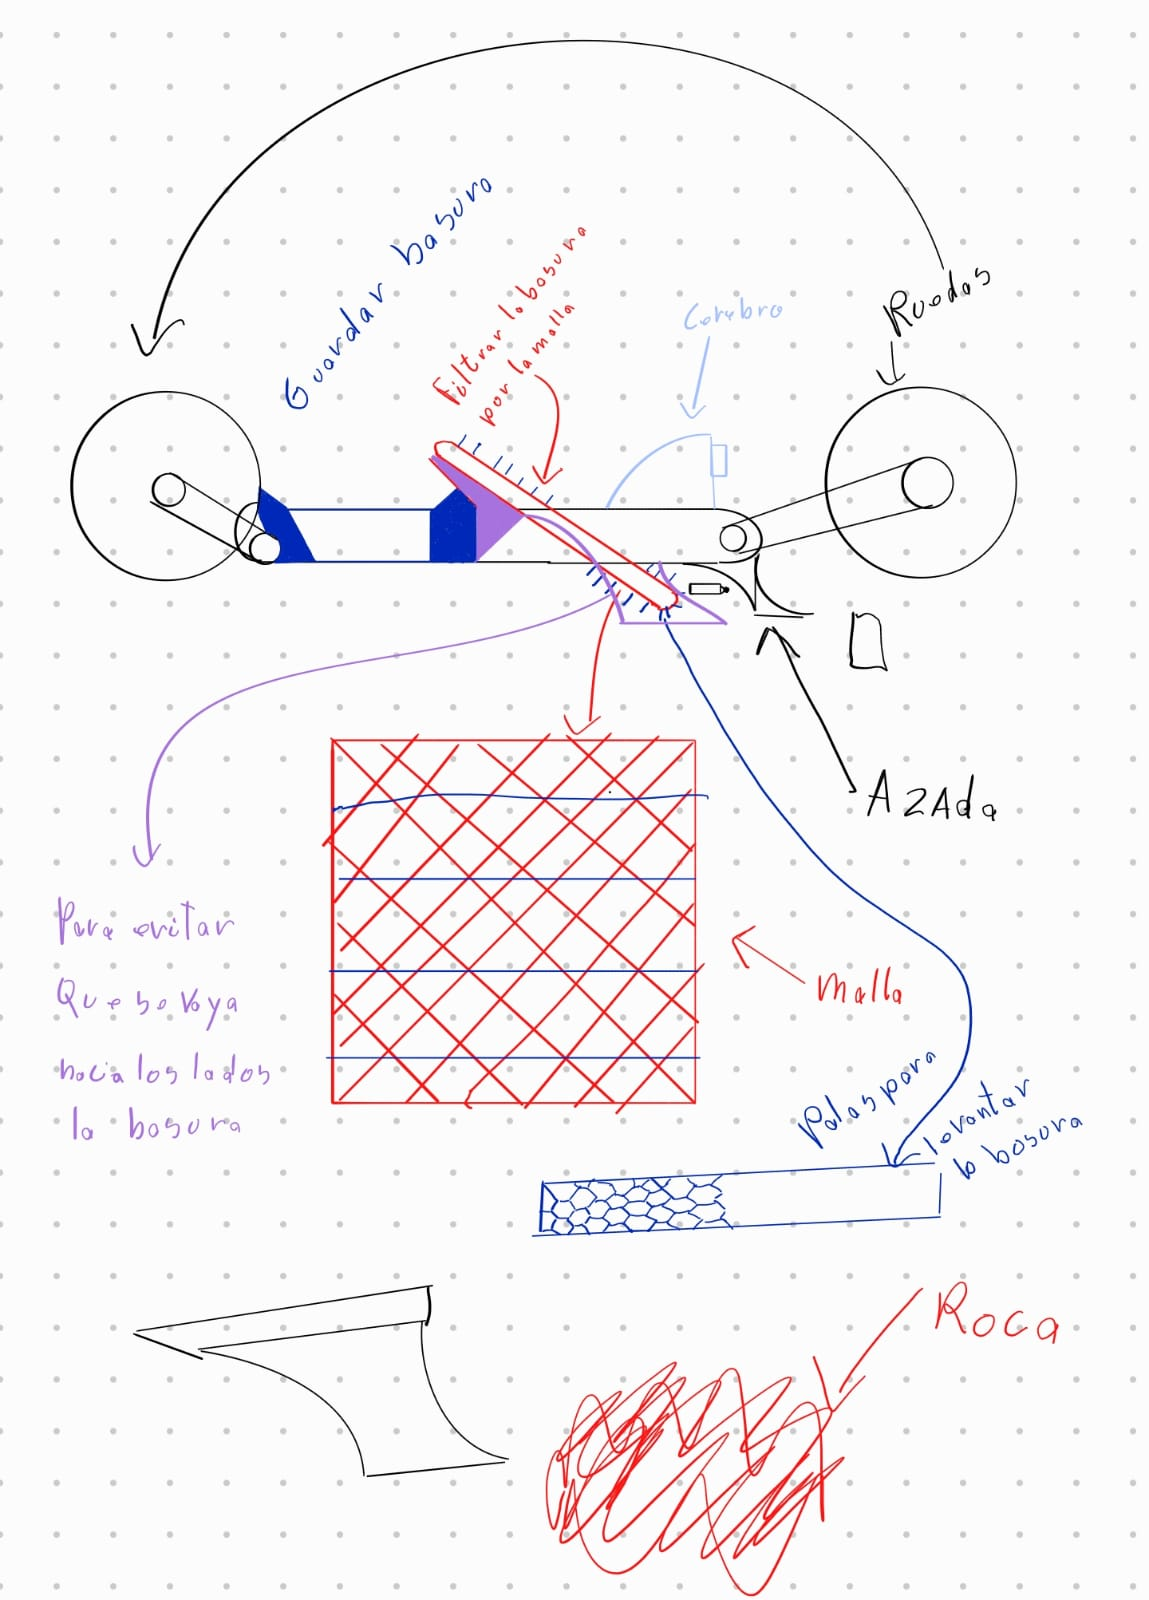
\includegraphics[width=\linewidth]{Boceto_1.jpeg}
    \caption{Boceto conceptual del sistema robótico Wallis con mecanismo de cribado subsuperficial.}
    \label{fig:boceto}
\end{minipage}
\hfill
\begin{minipage}{0.48\textwidth}
    \centering
    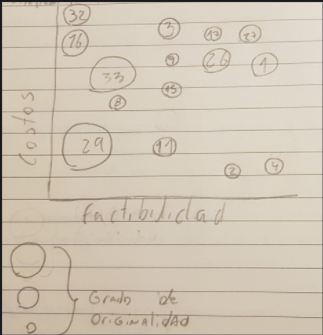
\includegraphics[width=\linewidth]{Comparacion.png}
    \caption{Evaluación de factibilidad y costo de alternativas de solución levantadas en el diagnóstico.}
    \label{fig:comparacion}
\end{minipage}
\end{figure}

% -------------------------------------------------------------------------
% ANEXO E: MATRIZ PESTEL Y BENCHMARKING DE SOLUCIONES
% -------------------------------------------------------------------------
\section{Análisis PESTEL y Matriz Atributos vs. Soluciones (Benchmarking)}
\label{anexo:pestel}

\noindent\textbf{1. Análisis PESTEL del Entorno Tecnológico y Ambiental}
\begin{itemize}[leftmargin=*, noitemsep]
    \item \textbf{Político:} Estrategias gubernamentales y de DIRECTEMAR para la conservación del borde costero; presión ciudadana sobre municipios para mantener playas seguras y certificadas.
    \item \textbf{Económico:} Pérdidas millonarias en el sector turismo por degradación costera (US\$60,7 millones según Oceana Chile \& Científicos de la Basura, 2026); inviabilidad económica para municipios chilenos de importar maquinaria extranjera pesada.
    \item \textbf{Social:} Creciente conciencia ecológica comunitaria; alta receptividad a dispositivos autónomos que operen en horarios nocturnos sin invadir el espacio recreativo diurno.
    \item \textbf{Tecnológico:} Disponibilidad de microcontroladores de bajo costo (ESP32), sensores ambientales y visión embebida (YOLOv8) que permiten robótica de servicio local y accesible (EcoMaker).
    \item \textbf{Ambiental:} Ambiente costero altamente agresivo con salinidad corrosiva, humedad y dinámica de mareas que exigen diseño estanco y materiales resistentes (PETG, acero inoxidable).
    \item \textbf{Legal:} Marco normativo favorable dado por la Ley 21.368 (plásticos de un solo uso), Ley 21.413 y ordenanzas municipales que sancionan botar basura en playas.
\end{itemize}

\vspace{0.2cm}
\noindent\textbf{2. Matriz de Atributos vs. Soluciones Existentes (Benchmarking)}
\begin{table}[h!]
\centering
\small
\setstretch{1.05}
\begin{tabularx}{\textwidth}{X c c c c}
\toprule
\textbf{Atributos Clave} & \textbf{Tractores Cribado} & \textbf{Voluntariados} & \textbf{Robots (BeBot)} & \textbf{Wallis (Propuesto)} \\
\midrule
Elimina basura enterrada (5--10 cm) & Sí & No & Parcial & \textbf{Sí} \\
No compacta la arena ni destruye dunas & No & Sí & Sí & \textbf{Sí} \\
Operación autónoma sin conductor & No & No & No (radio-control) & \textbf{Sí} \\
Operación nocturna desatendida & Rara vez & No & No & \textbf{Sí} \\
Bajo costo y adaptado a Chile & No ($>$US\$100k) & Sí & No (US\$60k) & \textbf{Sí ($<$US\$1.500)} \\
Capacidad de atrapar colillas y vidrios & Parcial & Mínima & Sí & \textbf{Sí} \\
\bottomrule
\end{tabularx}
\caption{Matriz comparativa de atributos entre soluciones existentes y el proyecto Wallis.}
\label{tab:benchmarking}
\end{table}

\end{document}
